\section{Connectivité Des Machines Virtuelles}

\begin{center}
    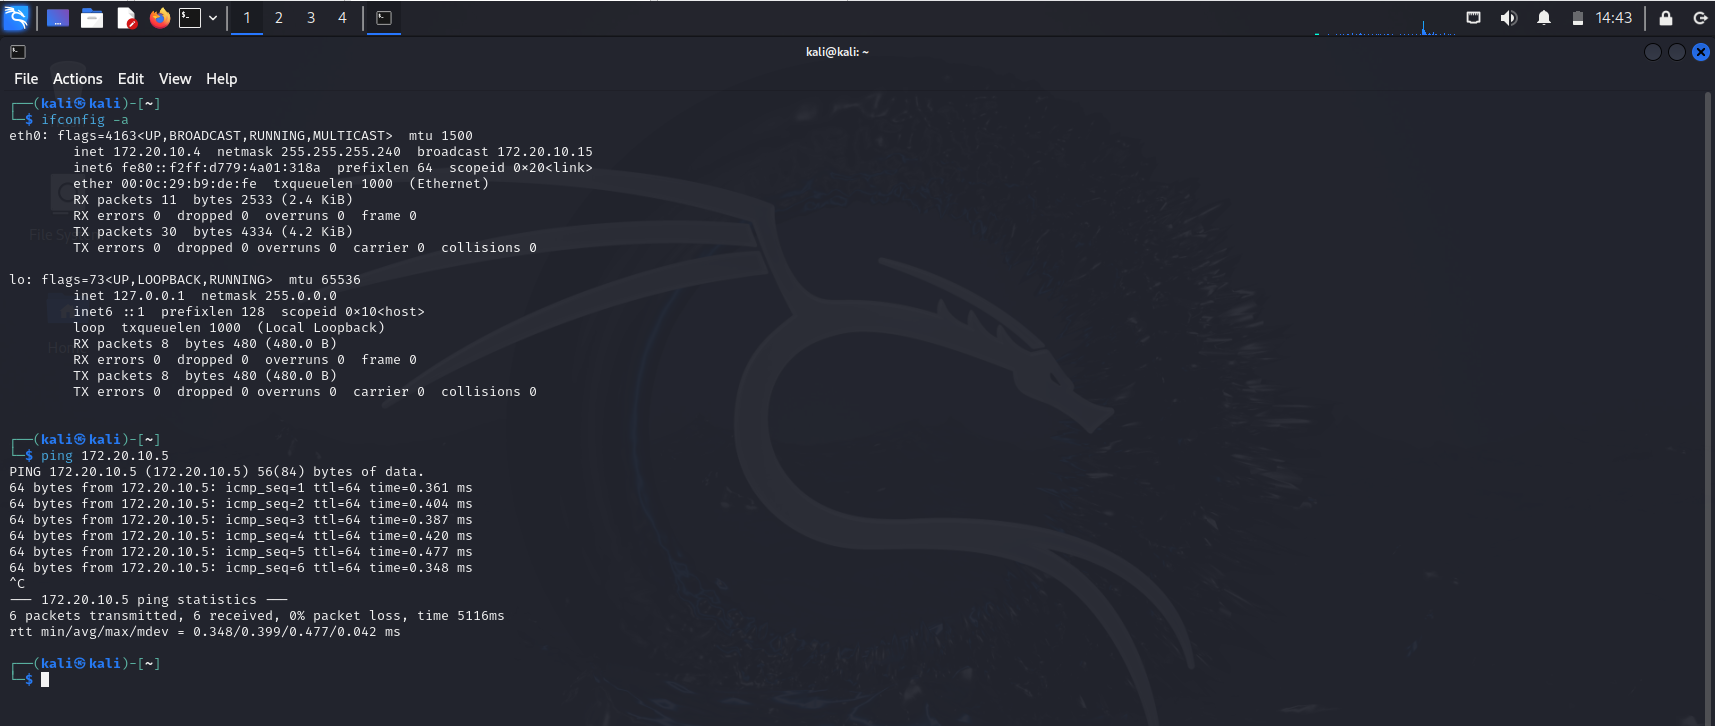
\includegraphics[width=0.8\textwidth]{Question/SC/ping1.PNG}
\end{center}

\vspace{0.25cm}

\begin{center}
    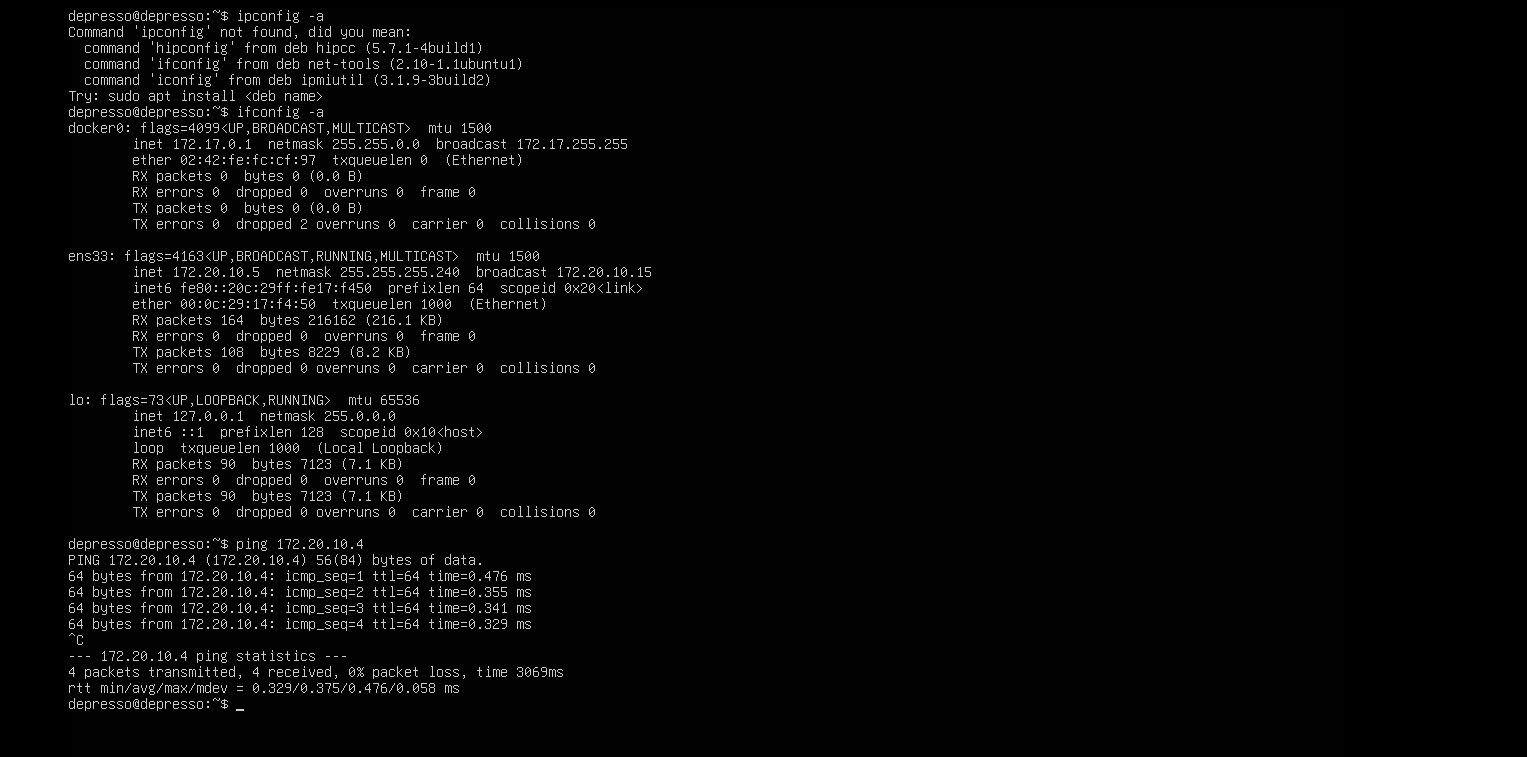
\includegraphics[width=0.8\textwidth]{Question/SC/ping2.PNG}
\end{center}

\vspace{0.35cm}

\begin{prettyBox}{Connectivité}{myblue}
D'après les captures d'écran, on remarque que les adresses IP des machines sont :
\begin{itemize}
    \item \textbf{Ubuntu : } \texttt{172.20.10.5}
    \item \textbf{Kali Linux : } \texttt{172.20.10.4}
\end{itemize}
Et le ping est réussi, donc il y a une connectivité.
\end{prettyBox}

